\documentclass[10pt]{article}
\usepackage[ngerman]{babel}
\usepackage[utf8]{inputenc}
\usepackage[T1]{fontenc}
\usepackage{graphicx}
\usepackage[export]{adjustbox}
\graphicspath{ {./images/} }
\usepackage{hyperref}
\hypersetup{colorlinks=true, linkcolor=blue, filecolor=magenta, urlcolor=cyan,}
\urlstyle{same}

\title{Modul Software-Entwicklung 1 (SWEN1) }

\author{Bachelor of Science (BSc) in Informatik}
\date{}


\begin{document}
\maketitle


\section*{LE 09 - Entwurf mit Design Pattern II Zusammenfassung}
SWEN1/PM3 Team:\\
R. Ferri (feit), D. Liebhart (lieh), K. Bleisch (bles), G. Wyder (wydg)

\section*{Lernziele LE 09 - Entwurf mit Design Patterns II}
\begin{itemize}
  \item Sie sind in der Lage:
  \item Den Aufbau der folgenden Design Patterns zu erklären und sie anzuwenden:
  \item Decorator
  \item Observer
  \item Strategy
  \item Composite
  \item State
  \item Visitor
  \item Facade
\end{itemize}

\textbackslash author\{

\begin{enumerate}
  \item Repetition Aufbau von Design Patterns \\
 2. Design Patterns \\
 3. Wrap-up und Ausblick\\
\}
\end{enumerate}

\section*{Repetition Aufbau Design Patterns}
\begin{itemize}
  \item Beschreibungsschema:
  \item Name
  \item Beschreibung Problem
  \item Beschreibung Lösung
  \item Hinweise für Anwendung
  \item Beispiele
  \item GRASP: Design Prinzipien
  \item GoF: Ausgefeiltere Spezialfälle von GRASP
\end{itemize}

\section*{1. Repetition Aufbau von Design Patterns \\
 2. Design Patterns \\
 3. Wrap-up und Ausblick }
\begin{itemize}
  \item Problem:
  \item Ein Objekt (nicht eine ganze Klasse) soll mit zusätzlichen Verantwortlichkeiten versehen werden.
  \item Lösung
  \item Ein Decorator, der dieselbe Schnittstelle hat wie das ursprüngliche Objekt, wird vor dieses geschaltet. Der Decorator kann nun jeden\\
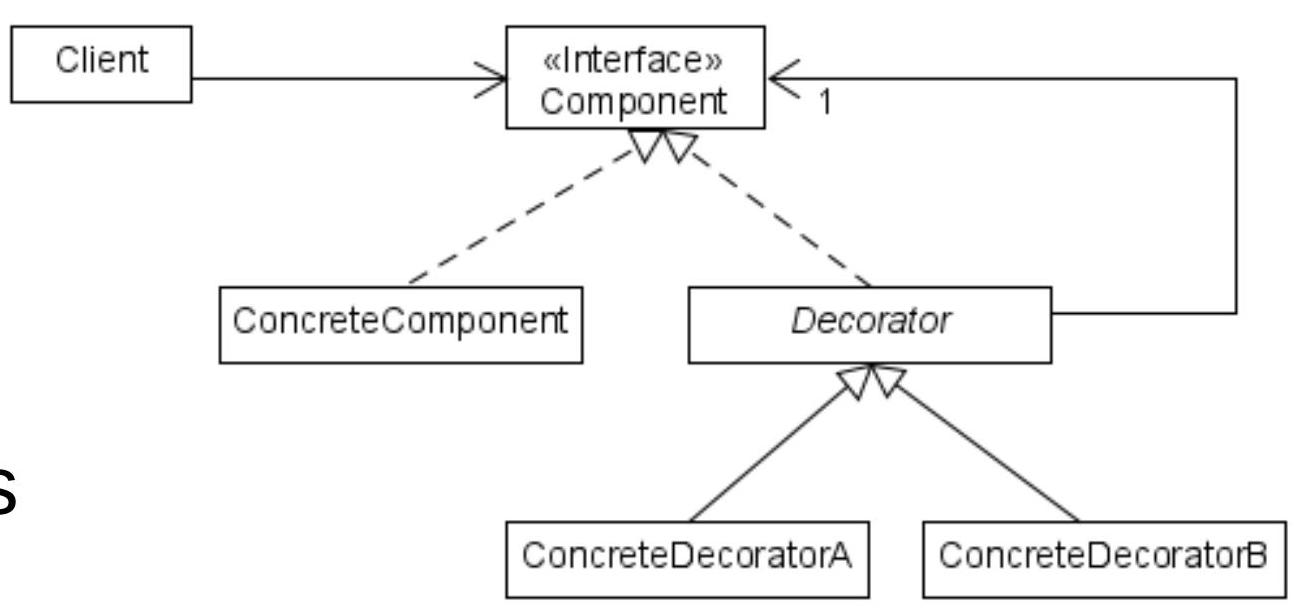
\includegraphics[width=\linewidth]{images/2025_01_02_110abbea2a944767a0afg-06} Methodenaufruf entweder selber bearbeiten, ihn an das ursprüngliche Objekt weiterleiten oder eine Mischung aus beidem machen.
  \item Hinweise
  \item Strukturell identisch mit dem Proxy Design Pattern, hat aber eine andere Absicht.
  \item Eigentlich identisch mit dem «Composite» Design Pattern, wenn die Anzahl Elemente 1 ist, hat aber natürlich auch eine andere Absicht.\\
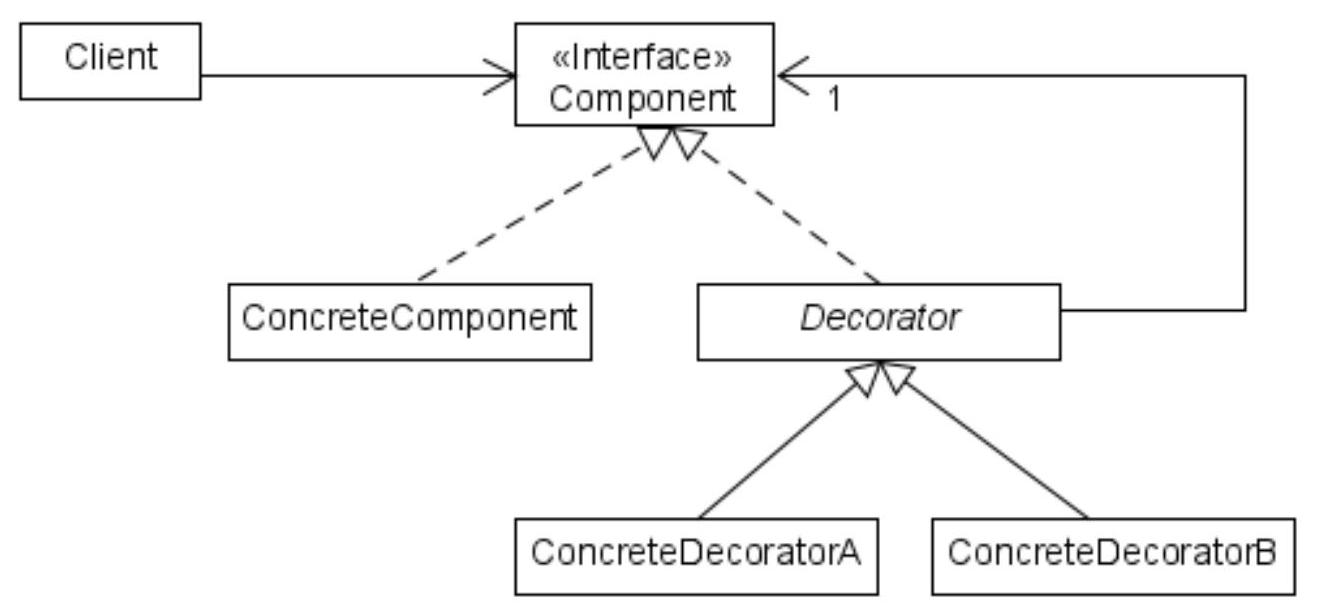
\includegraphics[width=\linewidth]{images/2025_01_02_110abbea2a944767a0afg-07}
  \item Problem:
  \item Ein Objekt soll ein anderes Objekt benachrichtigen, ohne dass es den genauen Typ des Empfängers kennt.
  \item Lösung
  \item Ein Interface wird definiert, das nur dazu dient, ein Objekt über eine Änderung zu informieren. Dieses Interface wird vom «Observer» implementiert. Das «Observable» Objekt benachrichtigt alle\\
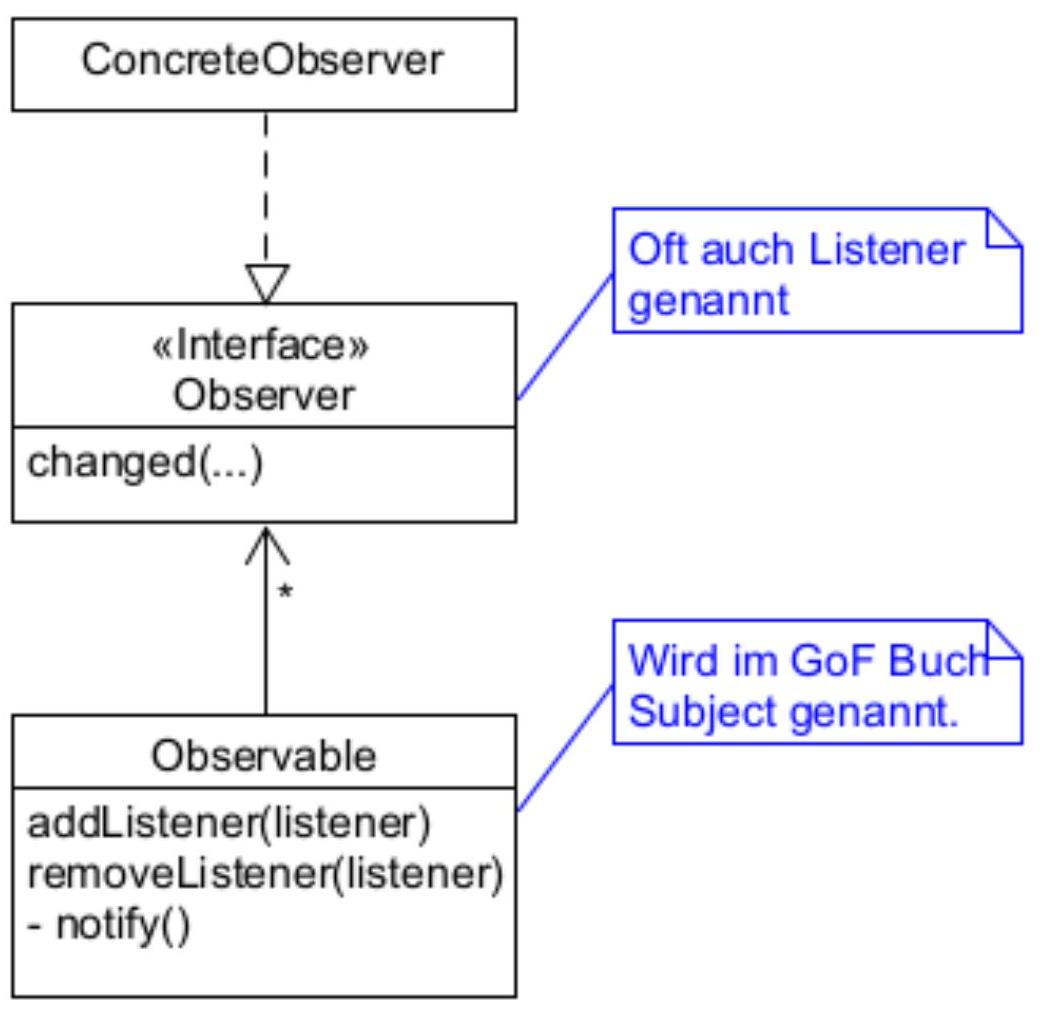
\includegraphics[width=\linewidth]{images/2025_01_02_110abbea2a944767a0afg-08} registrierten «Observer» über eine Änderung.
  \item Hinweise
  \item Oft wird dieses Pattern auch «PublishSubscribe» genannt.
  \item Observable kennt nur Observer, aber nicht den wahren Typ ConcreteObserver.
  \item 2 Phasen : Zuerst die Registrierung der Observer, dann die Benachrichtigungen durch das Observable.\\
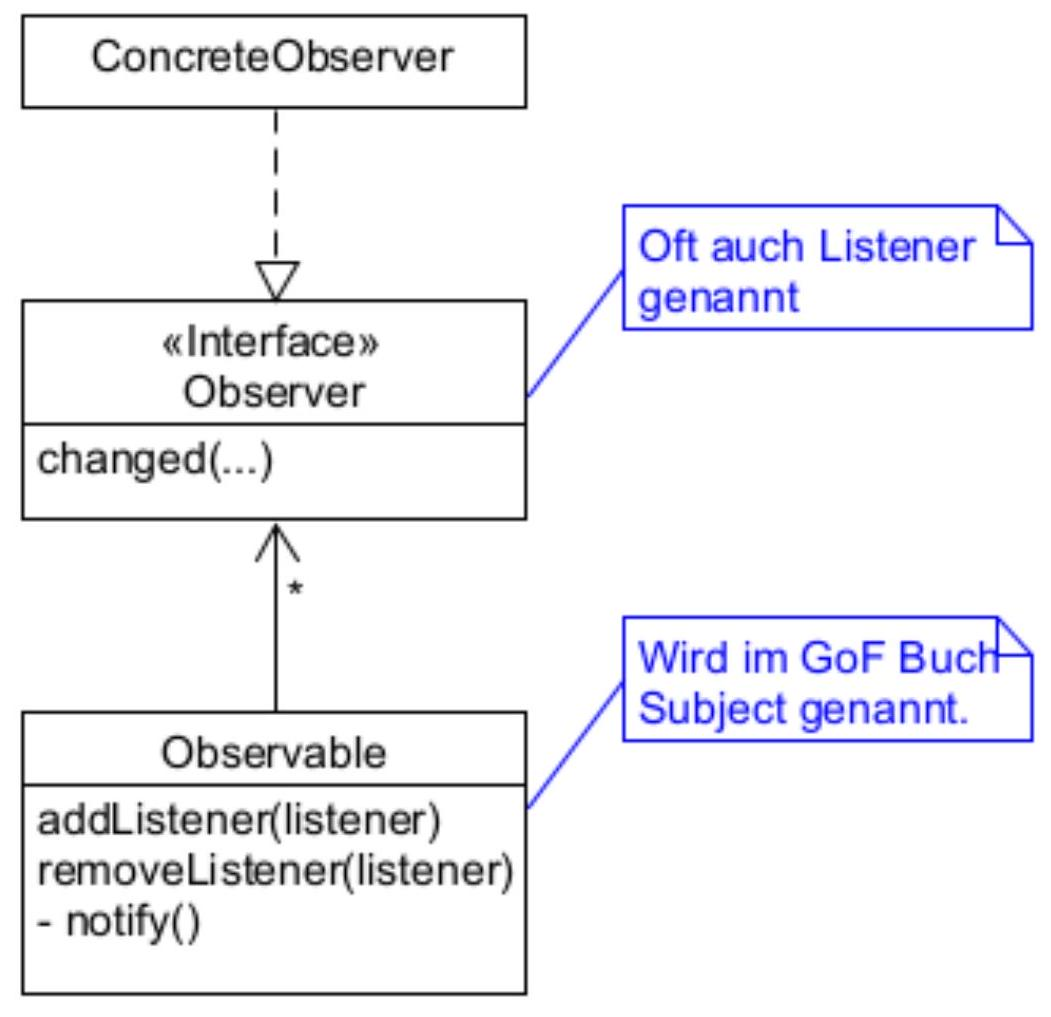
\includegraphics[width=\linewidth]{images/2025_01_02_110abbea2a944767a0afg-09}
\end{itemize}

\section*{Strategy: Problem und Lösung}
\begin{itemize}
  \item Problem:
  \item Ein Algorithmus soll einfach austauschbar sein.
  \item Lösung
  \item Den Algorithmus in eine eigene Klasse verschieben, die nur eine Methode mit diesem Algorithmus hat.
  \item Ein Interface für diese Klasse definieren, das von alternativen Algorithmen implementiert werden muss.
\end{itemize}

\section*{Strategy: Hinweise}
\begin{itemize}
  \item Hinweise
  \item Als Motivation für die einfache Austauschbarkeit können technische wie auch fachspezifische Gründe vorhanden sein.
  \item Das Interface hat nur eine einzige Methode. Als Parameter müssen alle Daten übergeben werden, die der Algorithmus benötigt. Dieser Parameter wird üblicherweise «context» benannt.\\
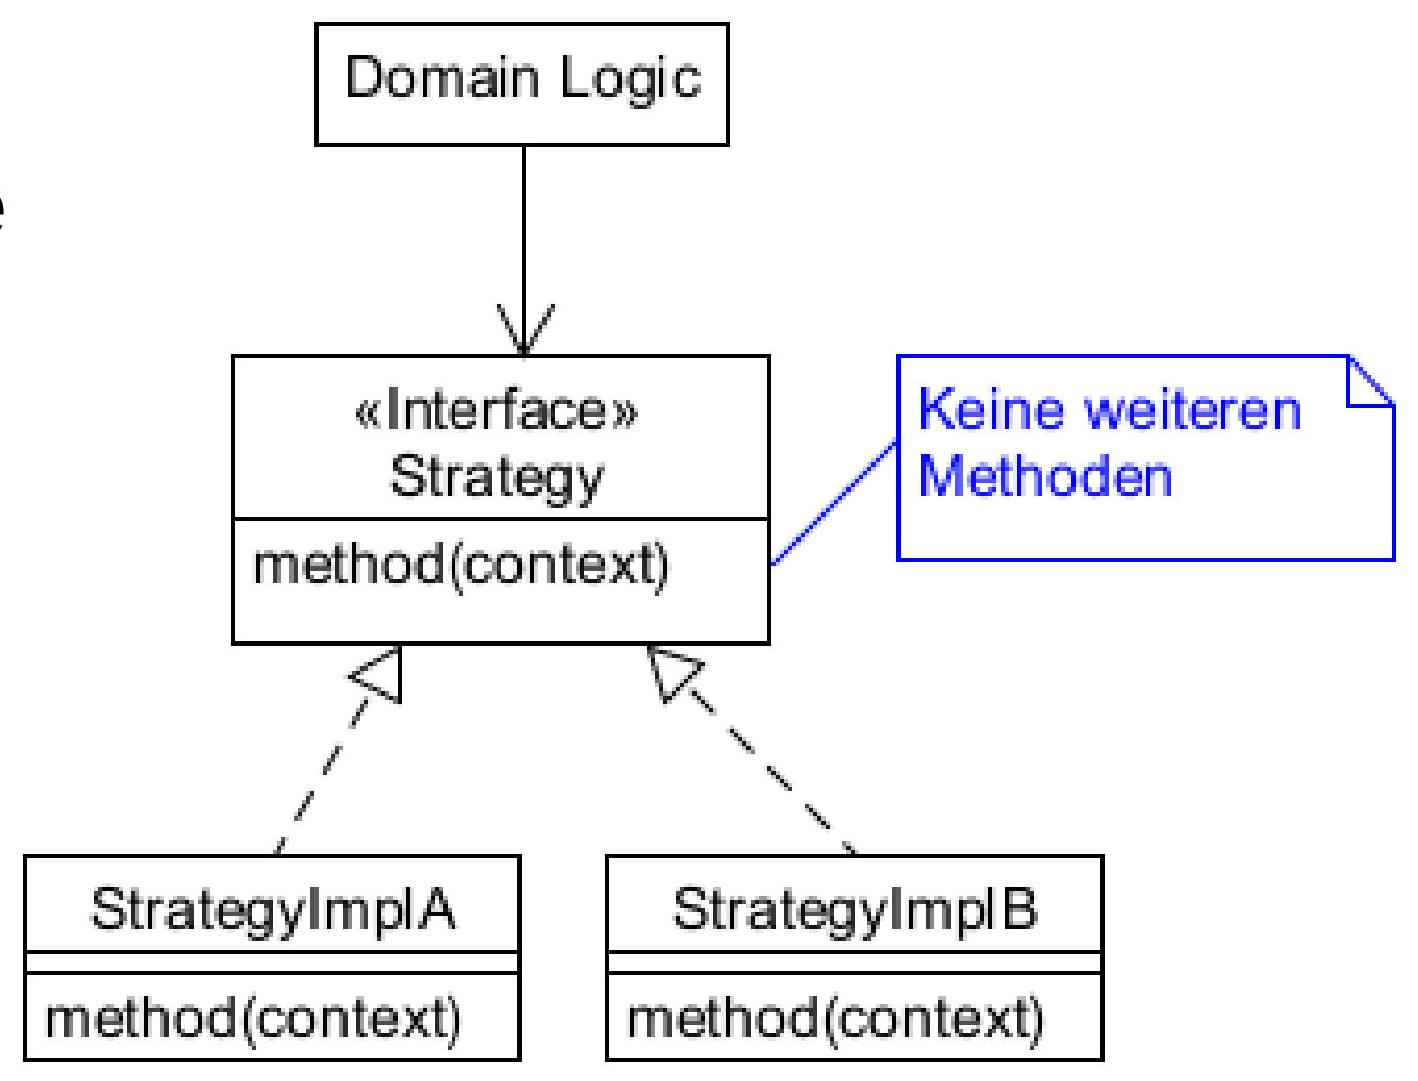
\includegraphics[width=\linewidth]{images/2025_01_02_110abbea2a944767a0afg-11}
\end{itemize}

\section*{Composite: Problem und Lösung}
\begin{itemize}
  \item Problem:
  \item Eine Menge von Objekten haben dasselbe Interface und müssen für viele Verantwortlichkeiten als Gesamtheit betrachtet werden.
  \item Lösung
  \item Sie definieren ein Composite, das ebenfalls dasselbe Interface implementiert und Methoden an die darin enthaltenen Objekte weiterleitet.\\
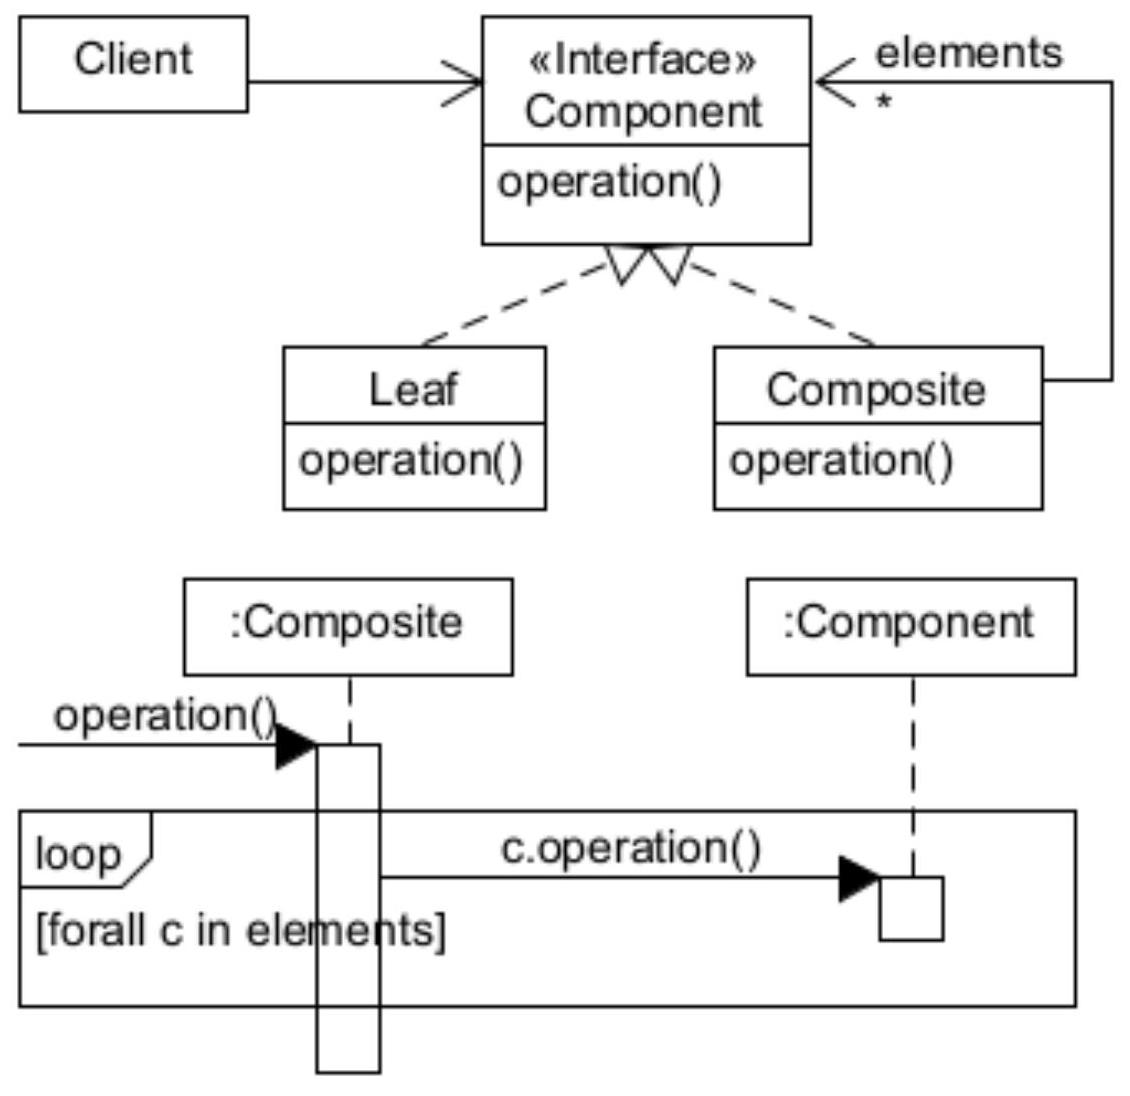
\includegraphics[width=\linewidth]{images/2025_01_02_110abbea2a944767a0afg-12}
\end{itemize}

\section*{- Hinweise}
\begin{itemize}
  \item Oft ist die hierarchische Struktur vom Fachgebiet her gegeben.
  \item Nicht alle Methoden delegieren einfach auf die enthaltenen Elemente. Vor- und Nachbearbeitung ist üblich, und gewisse Methoden müssen ganz anders implementiert werden.\\
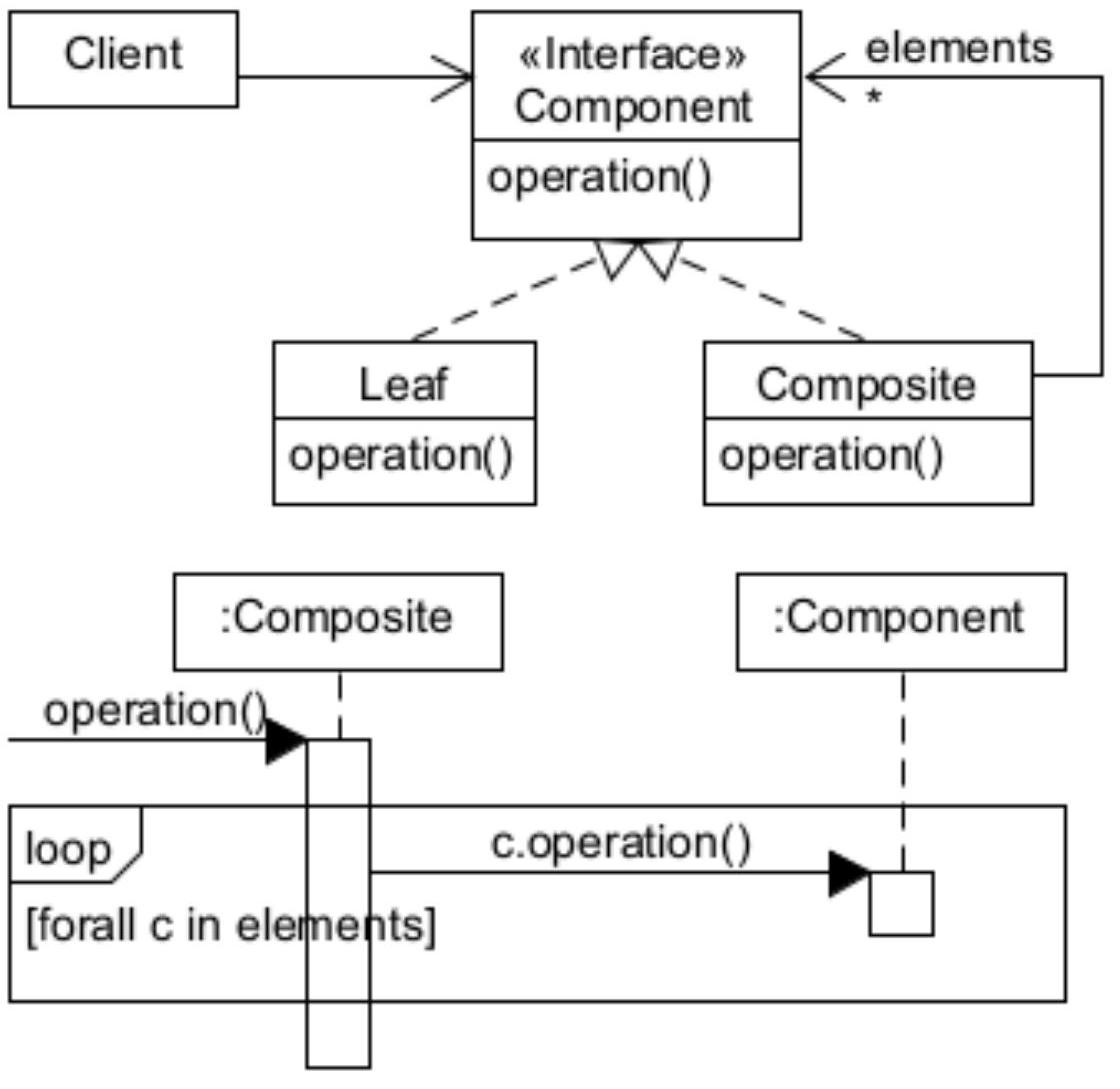
\includegraphics[width=\linewidth]{images/2025_01_02_110abbea2a944767a0afg-13}
\end{itemize}

\section*{State: Problem und Lösung}
\begin{itemize}
  \item Problem:
  \item Das Verhalten eines Objekts ist abhängig von seinem inneren Zustand.
  \item Lösung
  \item Das Objekt hat ein darin enthaltenes Zustandsobjekt.
  \item Alle Methoden, deren Verhalten vom Zustand abhängig sind, werden über das Zustandsobjekt geführt.
\end{itemize}

Zustandsabhängige Methoden werden weitergeleitet\\
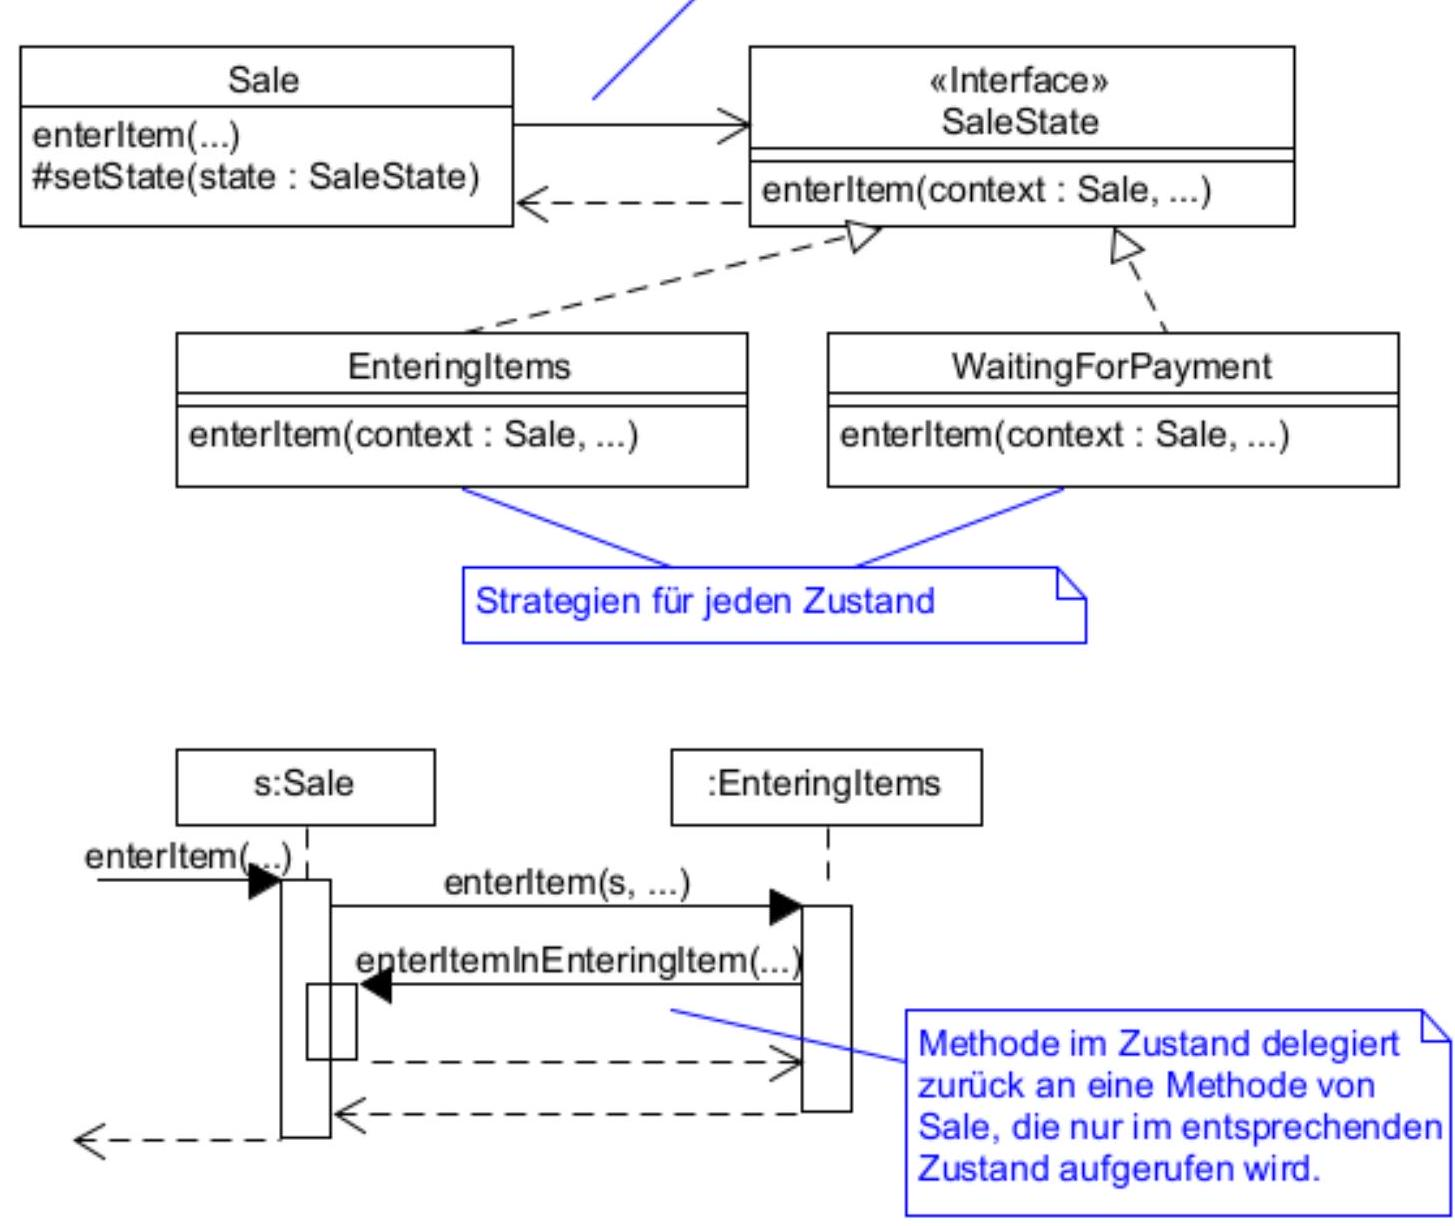
\includegraphics[width=\linewidth]{images/2025_01_02_110abbea2a944767a0afg-14}

\section*{- Hinweise}
\begin{itemize}
  \item Die Zustands-Klassen implementieren das Zustand-Interface.
  \item Die Zustands-Objekte sind nichts anderes als Strategy Objekte und können Singletons sein.
\end{itemize}

Zustandsabhängige Methoden werden weitergeleitet\\
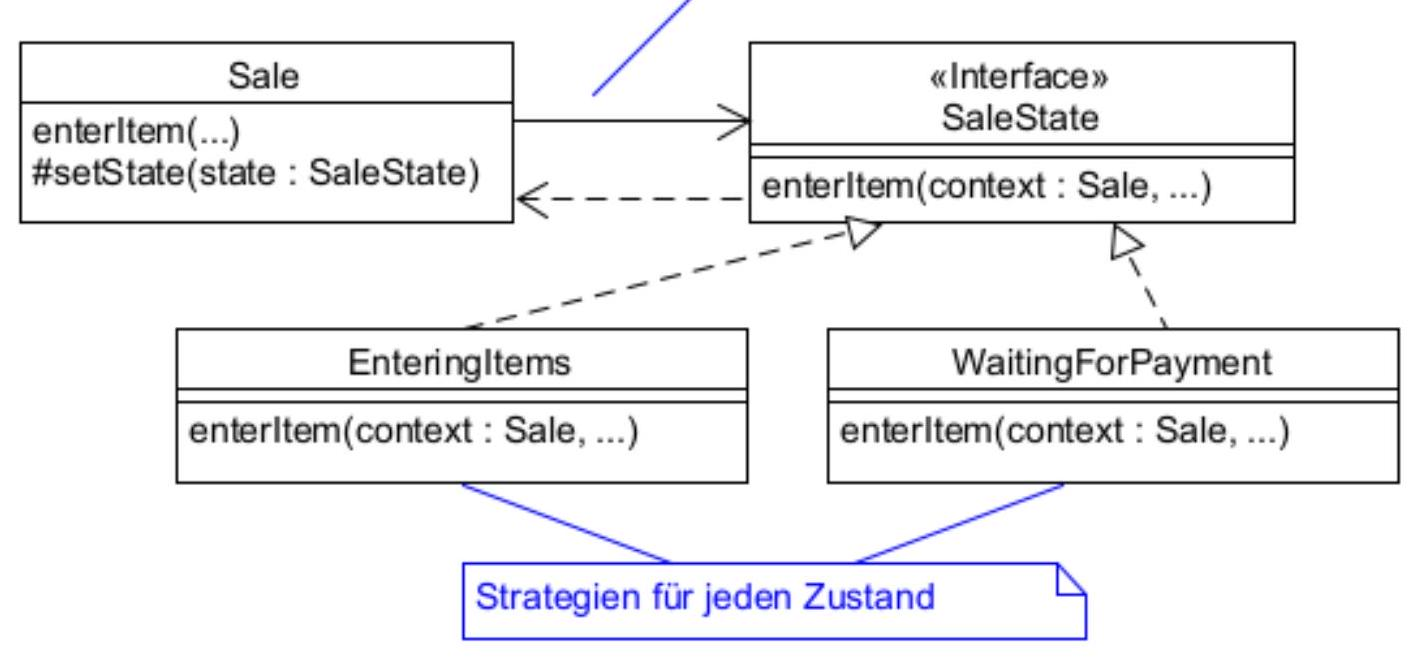
\includegraphics[width=\linewidth]{images/2025_01_02_110abbea2a944767a0afg-15(1)}

\begin{itemize}
  \item Das Zustandsobjekt hat entweder direkt den Code (als innere Klasse) oder delegiert an eine Methode des Objekts weiter.\\
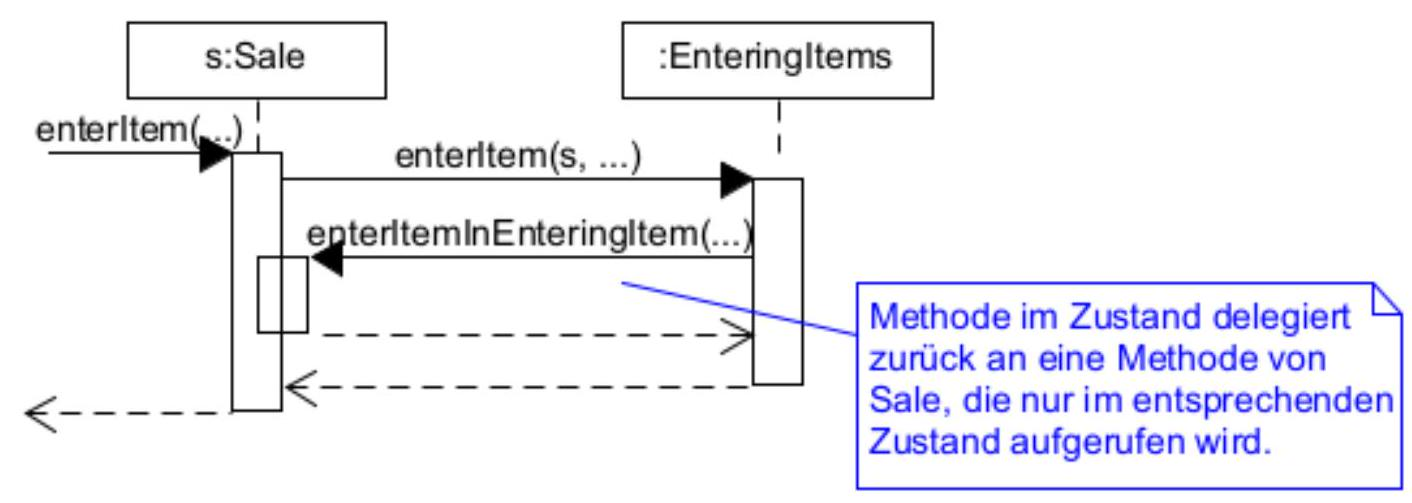
\includegraphics[width=\linewidth]{images/2025_01_02_110abbea2a944767a0afg-15}
\end{itemize}

\section*{Visitor: Problem und Lösung}
\begin{itemize}
  \item Problem:
  \item Eine Klassenhierarchie soll um (weniger wichtige) Verantwortlichkeiten erweitert werden, ohne dass viele neue Methoden hinzukommen.
  \item Lösung
  \item Die Klassenhierarchie wird mit einer Visitor-Infrastruktur erweitert. Alle weiteren neuen Verantwortlichkeiten werden dann mit spezifischen VisitorKlassen realisiert.\\
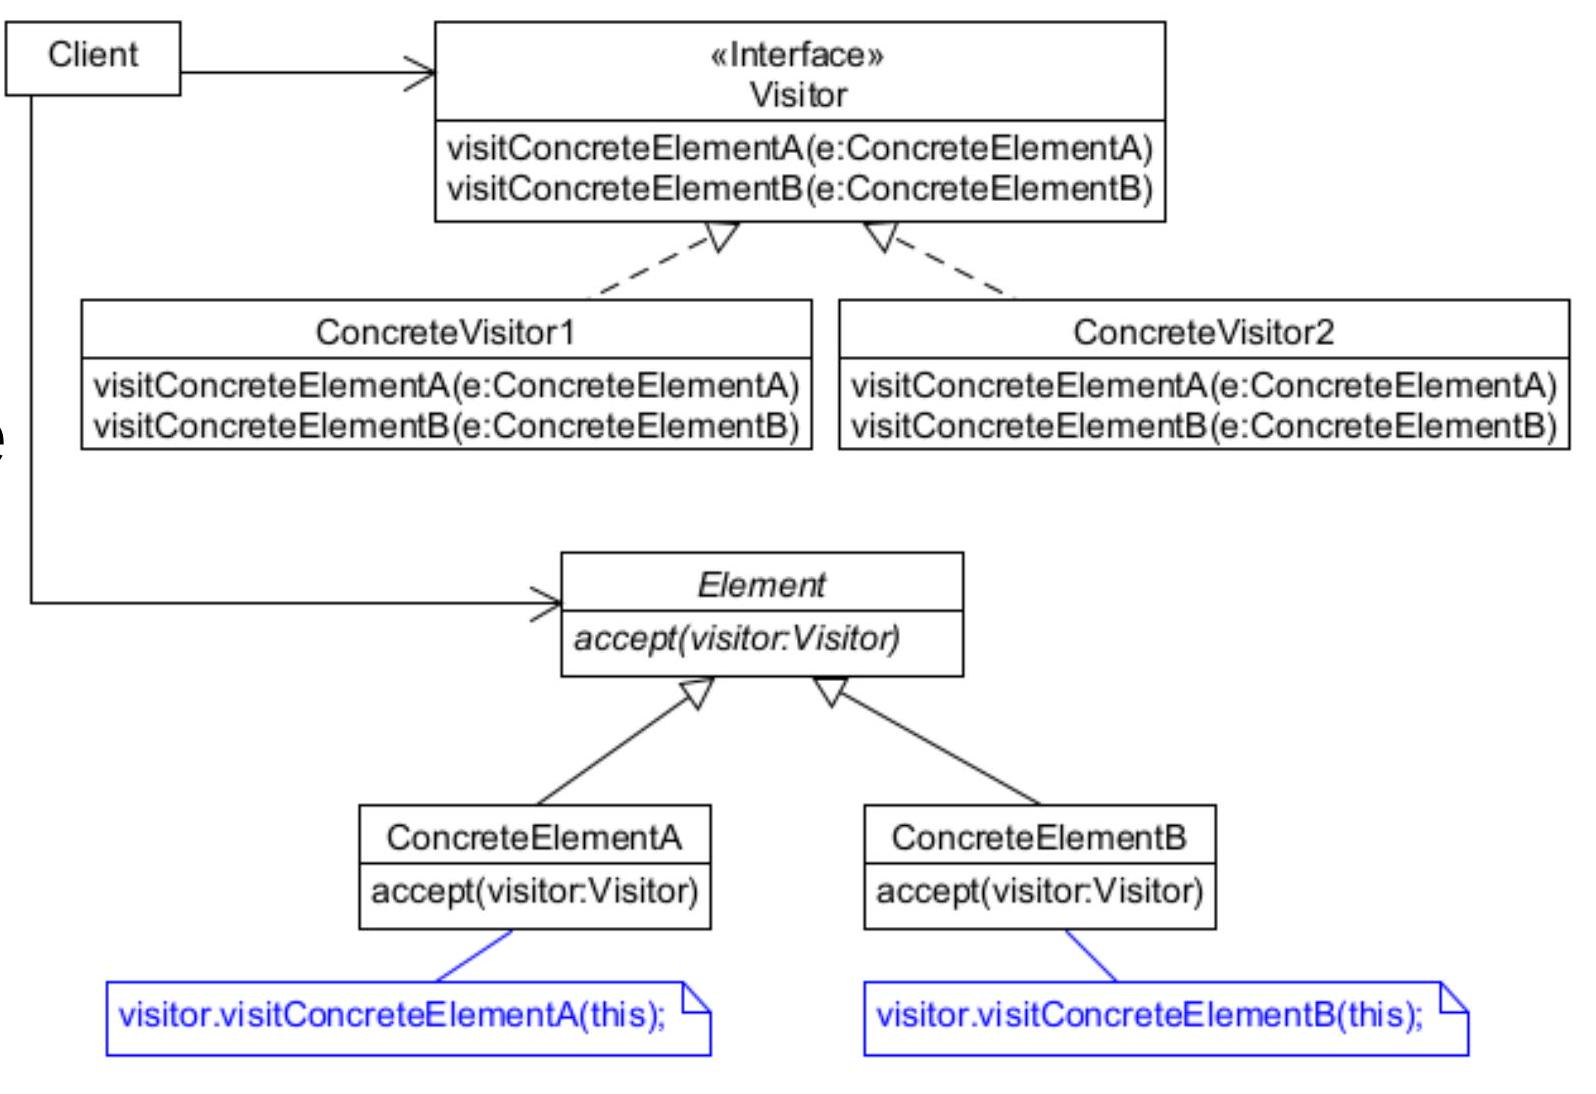
\includegraphics[width=\linewidth]{images/2025_01_02_110abbea2a944767a0afg-16}
\end{itemize}

\section*{Visitor: Hinweise}
\section*{- Hinweise}
\begin{itemize}
  \item Widerspruch zum Information Expert. Daher wichtige Methoden weiterhin direkt der Klasse hinzufügen.\\
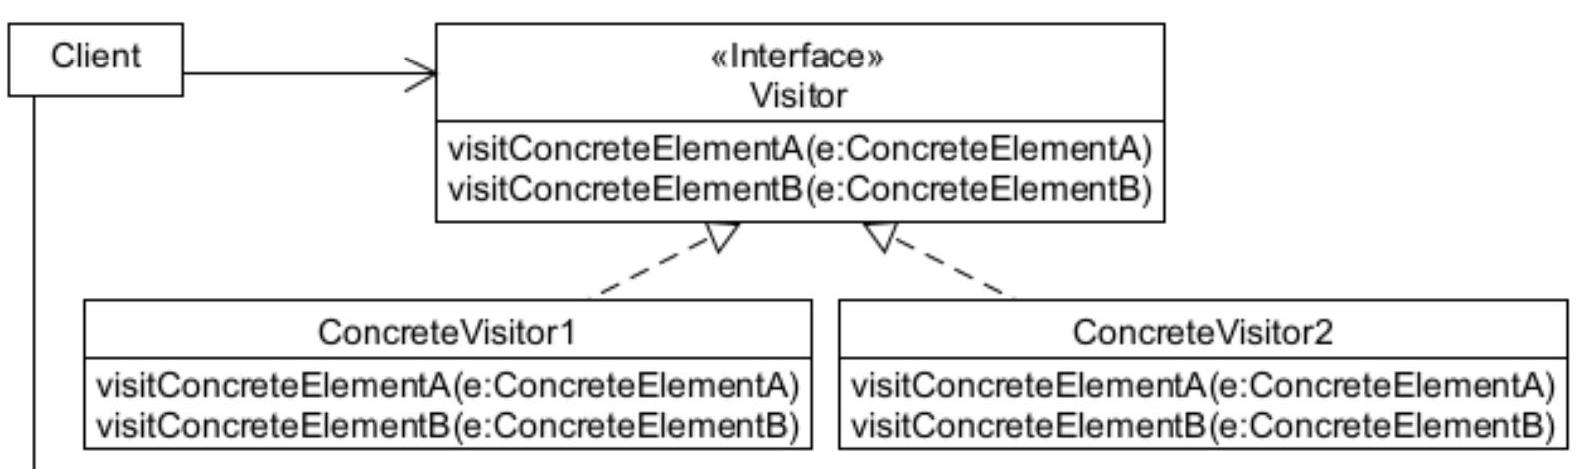
\includegraphics[width=\linewidth]{images/2025_01_02_110abbea2a944767a0afg-17}
  \item Oft werden Auswertungen an VisitorKlassen delegiert.
  \item Bei einer mehrstufigen Objekthierarchie stellt sich die Frage, wer die darin enthaltenen Elemente aufruft. Siehe Beispiel Schachprogramm.
  \item Problem:
  \item Sie setzen ein ziemlich kompliziertes Subsystem mit vielen Klassen ein. Wie können Sie seine Verwendung so vereinfachen, dass alle Team-Mitglieder es korrekt und einfach verwenden können?
  \item Lösung
  \item Eine Facade (Fassade) Klasse wird definiert, welche eine vereinfachte\\
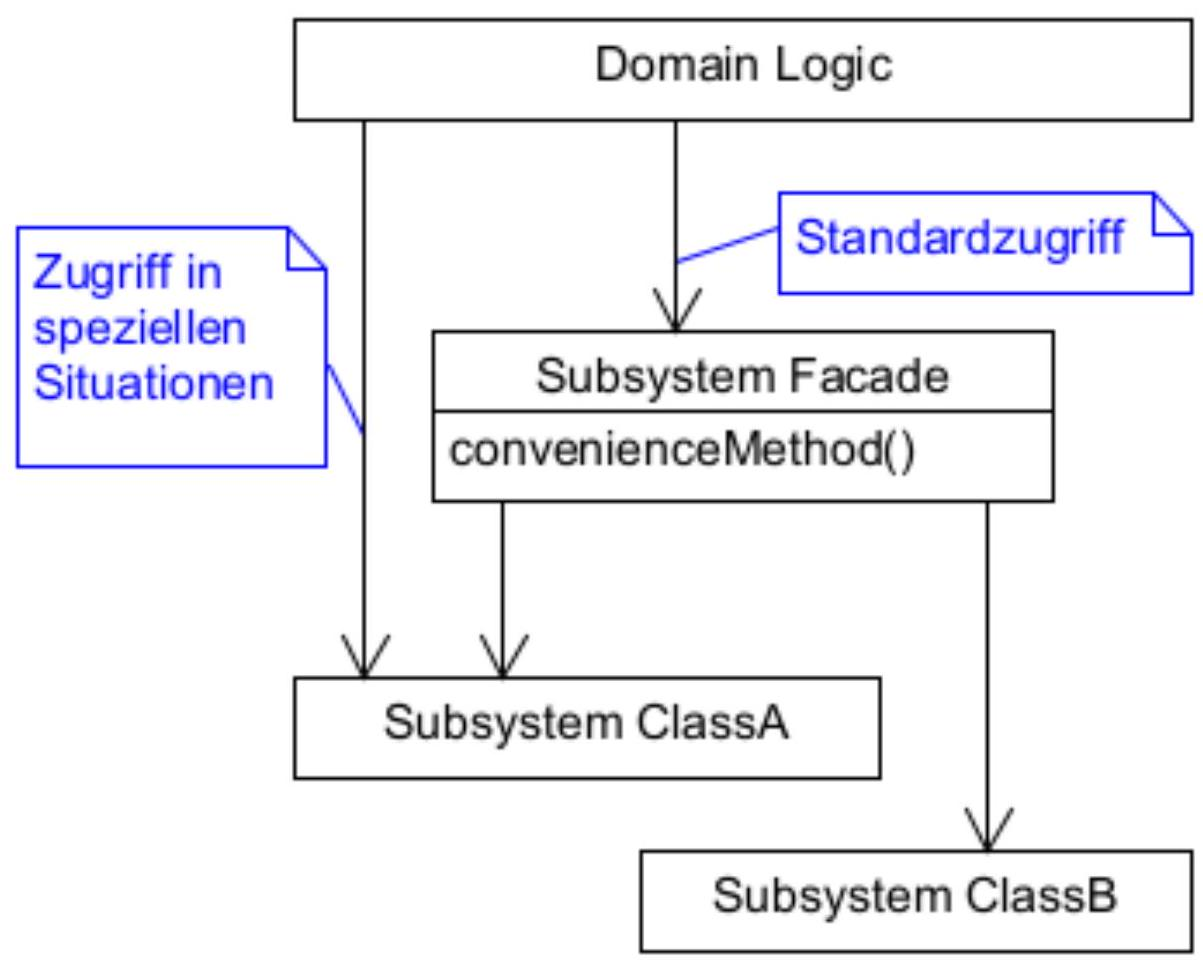
\includegraphics[width=\linewidth]{images/2025_01_02_110abbea2a944767a0afg-18} Schnittstelle zum Subsystem anbietet und die meisten Anwendungen abdeckt.
\end{itemize}

\section*{Facade: Hinweise}
\section*{- Hinweise}
\begin{itemize}
  \item Eine Facade kapselt, im Gegensatz zum Adapter, ein Subsystem nicht vollständig ab. Es ist erlaubt, dass die Methoden der Facade Parameter und Rückgabewerte haben, die Bezug auf das Subsystem nehmen.
  \item Wird oft vom Ersteller eines Frameworks\\
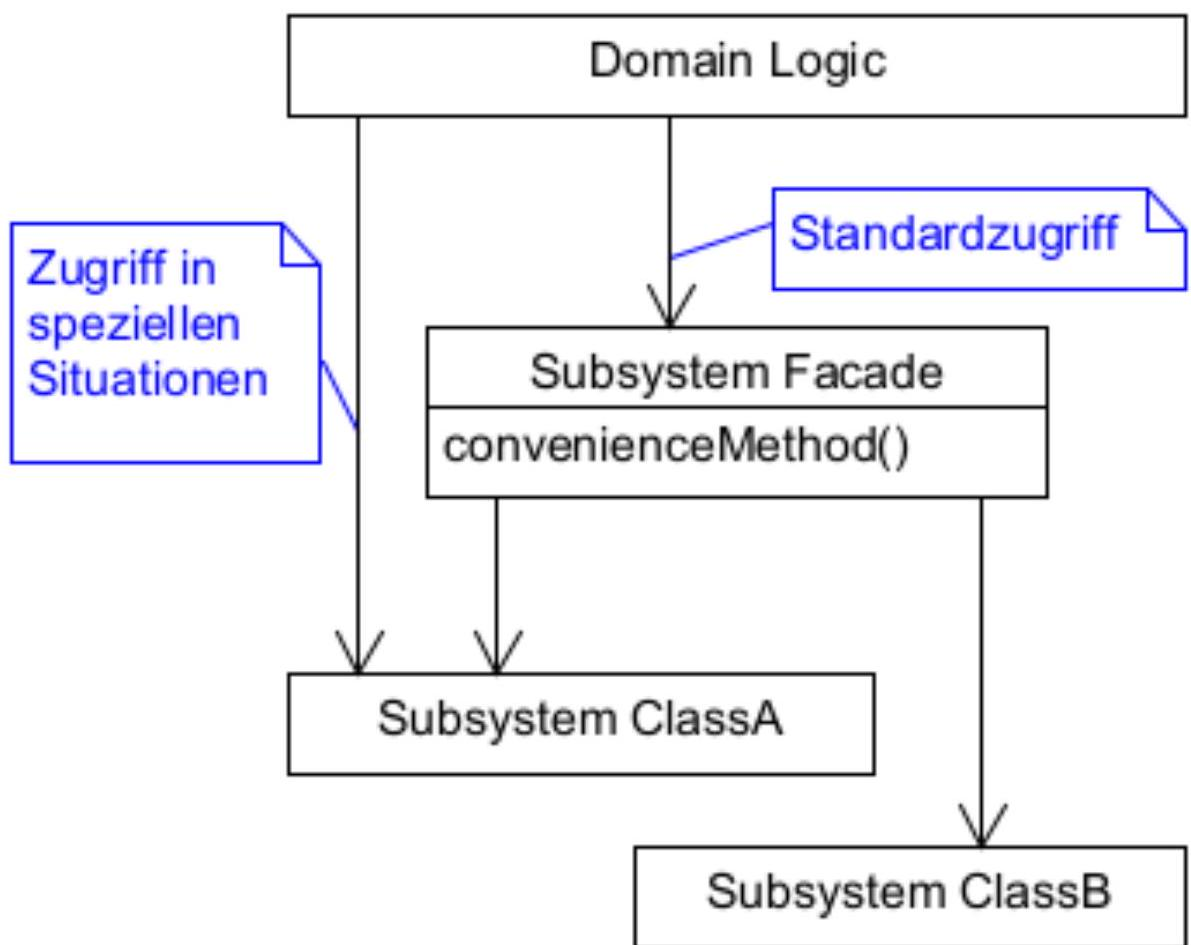
\includegraphics[width=\linewidth]{images/2025_01_02_110abbea2a944767a0afg-19}
\end{itemize}

\section*{1. Repetition Aufbau von Design Patterns \\
 2. Design Patterns \\
 3. Wrap-up und Ausblick }
\begin{itemize}
  \item Ein Decorator erweitert die Funktionalität eines Objekts (im Gegensatz zu Vererbung)
  \item Ein Observer beobachtet das Observable. Da der Observer dem Observable nur als Interface bekannt ist, wird Low Coupling unterstützt.
  \item Eine Strategy ist ein Klasse, die genau einen Algorithmus enthält. Über Polymorphismus kann dann die Strategy einfach ausgetauscht werden.
  \item Ein Composite beinhaltet Objekte, die dasselbe Interface wie das Composite implementieren. Viele Methoden werden dann auf diese Objekte weitergeleitet.
  \item Zustandsabhängiges Verhalten wird über ein State Objekt geleitet.
  \item Ein Visitor besucht Objekte, die dann die richtige Methode auf dem Visitor aufrufen.
  \item Ein Facade bietet für ein Teilsystem eine vereinfachte Benutzung an.
  \item In der nächsten Lerneinheit werden wir:
  \item Einen Quiz zum Design durchführen.
  \item Den Prozess des Refactorings genauer anschauen.
\end{itemize}

\section*{Quellenverzeichnis}
[1] Larman, C.: UML 2 und Patterns angewendet, mitp Professional, 2005\\[0pt]
[2] Seidel, M. et al.: UML @ Classroom: Eine Einführung in die objektorientierte Modellierung, dpunkt.verlag, 2012\\[0pt]
[3] Martin, R. C.: Clean Architecture: A Craftsman's Guide to Software Structure and Design, mitp Professional, 2018\\[0pt]
[4] Gamma, E et al.: Design Patterns: Elements of Reusable Object-Oriented Software Addison Wesley Longman, 1995\\[0pt]
[5] McDonald, J: DZone Refcardz: Design Patterns, \href{http://www.dzone.com}{www.dzone.com}, 2008


\end{document}